 \chapter{The ATLAS Detector at the Large Hadron Collider}%
\label{ch:detector}

\section{The Large Hadron Collider}%
\label{sec:lhc}%
The Large Hadron Collider (LHC)~\cite{LHC-dr} is a large circular machine
located 100~m underground straddling the Swiss-French border at the European
Organisation for Nuclear Research (CERN). The LHC accelerates and collides
protons and other charged particles. It has a circumference of 27~km and resides
in a tunnel which was originally excavated for the Large Electron-Positron
Collider~\cite{LEP} experiment. During its construction the tunnel was the
largest civil engineering project in Europe to date. Today there are many
physics experiments that take place at CERN, some of which are marked in
figure~\ref{fig:lhc-acc}. There are currently seven experiments that record
data from the collisions at the LHC: ATLAS~\cite{ATLAS-loi}, CMS~\cite{CMS-loi},
LHCb~\cite{lhcb-loi}, ALICE~\cite{ALICE-loi}, MoEDAL~\cite{MoEDAL-loi},
TOTEM~\cite{TOTEM-loi} and LHCf~\cite{lhcf-loi}.
\begin{figure}[ht]
  \centering
  \includegraphics[width=.9\textwidth]{lhc-accelerator}
  \caption[The CERN accelerator complex]{The CERN accelerator
    complex~\cite{LHC-acc-fig}.}%
  \label{fig:lhc-acc}
\end{figure}

% The Lorentz force is fundamental to the LHC's accelerator technologies and
% detectors. Expressed as
% \begin{equation}
%   \label{eq:lorentz}
%   \vec{F} = q(\vec{E} + \vec{v} \times \vec{B}),
% \end{equation}
% it is clear that the force due to an electric field $\vec{E}$ on a particle with
% charge $q$ acts in the direction of the velocity of the field whereas the force
% due to a magnetic field $\vec{B}$ acts perpendicular to both the field and the
% velocity of the particle $\vec{v}$. It is therefore clear that an electric field
% may be used to accelerate and give energy to a charged particle whereas a
% magnetic field will alter the trajectory of a particle whilst keeping its energy
% constant.

The LHC is a synchrotron, an accelerator that uses magnets in a dipole
configuration, such as in figure~\ref{fig:dipole}, to bend the path of charged
particles into conformity with its circular shape. It is apparent from studying
the figure that counter-rotating beams of same sign charged particles will
require two sets of dipole magnets in order to rotate in opposite directions
around the same ring. This is one disadvantage of a proton-proton collider with
respect to a proton-anti-proton collider such as the Tevatron~\cite{tevatron-01}
which can use the same magnets for both beams. On the other hand, the
proton-proton collider is able to separate the beams after they have been
brought together to collide with a single dipole. The bending magnets of a
synchrotron are designed to ramp up their magnetic field in synchronisation
with the kinetic energy of the accelerated particles, allowing higher energies
to be achieved before the beam is lost. The LHC can accelerate each beam to an
energy of 6.5~TeV, leading to collisions with a centre of mass energy of
$\sqrt{s} = 13 $~TeV, although the design energy of the LHC is $\sqrt{s} = 14
$~TeV. The Tevatron held the previous record for centre of mass energy of
collisions of $\sqrt{s} = 2 $~TeV. The LHC has 1232 dipole magnets~\cite{LHC-dr}
which are made of copper-clad niobium-titanium cables, a superconducting
material whose electrical resistance falls to zero below $10$~K. In order to
maintain super-conductivity a cryogenic system using liquid helium is employed
to cool the magnets. The higher the velocity of a charged particle, and the
tighter the desired bending radius, the larger the magnetic field required to
perform the bending. The large size of the LHC and the choice of superconducting
magnet technologies are both informed by the aim to accelerate protons to the
highest energy, and therefore velocity, possible.
\begin{figure}[ht]
  \centering
  \includegraphics[trim={1cm 1cm 1cm 1cm}, clip, width=.6\textwidth]{uniform_gap}
  \caption[Magnets in a dipole configuration.]{A representation of a pair of
    idealised cylindrical magnets in a dipole configuration. Two positively
    charged particles are shown as circles, the red particle is traveling out of
    the page, the green particle is traveling into the page. The forces
    experienced by each particle due to the magnetic field are shown as blue
    arrows.}
  \label{fig:dipole}
\end{figure}


The force which accelerates the particles is provided by radio-frequency
cavities, of which the LHC has 16~\cite{LHC-dr} The electric field in the
radio-frequency cavity forms a standing wave, the separation between bunches of
particles to be accelerated must be matched to the frequency of this wave.
Protons in the LHC are accelerated in bunches and in vacuum, to increase
the likelihood of collisions and mitigate loss of energy and scattering effects
due to interactions with air molecules. These two factors lead to the occurrence
of space charge which causes an increase in the emittance of the beam, where the
emittance is defined as the total area that the beam occupies in its beam-pipe.
The greater the energy of the particles the more they can overcome increase in
emittance due to space charge. Increased emittance is especially problematic in
circular accelerators where periodic effects can quickly lead to the loss of
beam. For these reasons it would be very challenging to accelerate protons from
rest in a synchrotron. The starting point for the protons of the LHC is
therefore a linear accelerator called Linac2 which is used to overcome space
charge effects before the protons move on to a series of synchrotrons as seen in
figure~\ref{fig:lhc-acc}.

Even a beam with its emittance under control would still be lost from the
accelerator if only dipole magnets were used to control its path. Magnets in a
quadrupole configuration as in figure~\ref{fig:quadrupole} are used to focus the
beam and keep it in the beam-pipe. The quadrupoles behave such that particles
feel a force that increases with the distance from the centre of the beam
leading to simple harmonic motion of individual particles in a bunch. The LHC
has a series of 24 quarupole magnets each for focusing in the horizontal and vertical
directions~\cite{LHC-dr} as well as higher multipole configurations;
sextupole, octupole, decapole and dodecapole which are used to correct
imperfections in the fields of other magnets.
\begin{figure}[ht]
  \centering
  \includegraphics[trim={0 0.7cm 0 0.5cm}, clip,
  width=.6\textwidth]{quarupole_with_beamspot}
  \caption[Magnets in a quadrupole configuration.]{Representation of an
    idealised set of coil magnets in a quadrupole configuration with a proton
    beamspot shown as a red ellipse. The proton beam is drawn coming out of the
    page (\emph{watch out!}), magnetic field lines are drawn in black and the
    forces acting on each bunch of protons are drawn as blue arrows.}
  \label{fig:quadrupole}
\end{figure}

% The LHC receives protons that have already been accelerated somewhat by the
% Super Proton Synchrotron (SPS), another of the accelerators at the CERN
% accelerator complex shown in figure~\ref{fig:lhc-acc}. The circular design of
% both the LHC and SPS allows protons to be accelerated many times around their
% respective rings until their velocity is fast enough for a high energy
% collision. The highest energy collisions achieved take place at a centre of mass
% energy of $\sqrt{s} = 13 $~TeV, although the design energy of the LHC is
% $\sqrt{s} = 14 $~TeV. Despite having not yet reached its design energy the LHC
% collides particles with the highest energy of any particle collider in history
% and is currently alone at the energy frontier of modern physics. At the time of
% writing the LHC is in it's second long shutdown during which maintenance and
% upgrades to the LHC and the particle detectors located around its ring take
% place. The LHC has completed two runs data taking from collisions, Run 1 took
% place from 2009 to 2013, followed  by Run 2
% between 2015 and 2018. The period between runs is known as long shutdown 1 (LS1), and
% was used to perform maintenance and upgrades. Many analyses from Run 1 have been
% published including, most notably the discovery of the Higgs
% boson~\cite{DiscoHiggsATLAS, DiscoHiggsCMS}. Some Run 2 analyses have also
% published results a highlight of which is LHCb's discovery of charge parity
% violation in charm decays~\cite{cp-charm}. Despite these impactful results there
% are many more results expected from the LHC experiments as data continues to be
% analysed.

Ignoring systematic uncertainties for the moment, the sensitivity of a
measurement can be increased by having a larger dataset, in this case more
recorded collisions. Constraints on the number of years the LHC is able to run
for mean that the best way to record more collisions is to collide more
particles per second. A quantity known as the luminosity is often used to
describe how much data is available for an analysis, written as
\begin{equation}
  \label{eq:luminosity} L = \frac{1}{\sigma}\frac{dN}{dt},
\end{equation} where $\sigma$ is the cross-section, an area within which
particles must pass by one another in order to interact, and $N$ is the number
of events recorded in a period of time $t$. For luminosity at the LHC $N$ can be
expressed as
\begin{equation}
  \label{eq:lhc-lumi} \frac{dN}{dt} = n_{bp}n_{1}n_{2}\nu_{r},
\end{equation} where $n_{bp}$ is the number of colliding bunch pairs, $n_{1}$
and $n_{2}$ are the number of protons in each beam and $\nu_r$ is the frequency
with which the beams rotate around the LHC's circumference. The number of
particles in the beams is limited by space charge. The number of bunches is
limited by the frequency that the radio-frequency cavities can operate at. The
revolution frequency is limited by the strength of the dipole magnets and the
circumference of the accelerator ring. Increasing luminosity by reducing the
cross-section amounts to reducing the beam widths which is limited by the
emittance of the beam. The LHC has already exceeded its design luminosity
providing physicists with more data to analyse than expected and plans are well
underway for the upgrade to a High-Luminosity LHC (HL-LHC)~\cite{hilumi-tdr}.

\section{The ATLAS Detector}%
\label{sec:atlas}

The ATLAS detector~\cite{ATLAS} resides at a location on the LHC ring called
Point 1, its full name is A Toroidal LHC ApparatuS. A diagram of the detector is
shown in figure~\ref{fig:ATLAS-det}. ATLAS is considered to be a general purpose
particle detector and has a wide physics programme, including: Higgs boson physics,
top quark physics, searches for Supersymmetry and exotic states, probes of CP
violation in b-quarks and light states and heavy ion physics. The detector
itself is very large in size, spanning a width of 25~m and a length of 44~m and
weighs 7000~tonnes which is comparable to the weight of the wrought iron content
of the Eiffel tower~\cite{Eiffel-weight}.
\begin{figure}[ht]
  \centering
  \includegraphics[width=.85\textwidth]{ATLAS-detector}
  \caption[The ATLAS Detector]{Computer generated image of the whole ATLAS
    detector with the major sub detectors labeled~\cite{ATLAS-det-fig}.}%
  \label{fig:ATLAS-det}
\end{figure}


Due to the composite nature of the proton, the decay products of collisions are
extremely numerous. Additionally, when two bunches of protons cross, there is the
chance that more than one hard scattering event occurs and softer glancing
collisions are also a possibility. The number of hard scattering events in a
given bunch crossing is known as the pile-up of the collision and is often
denoted with the symbol $\mu$. As can be seen by inspecting
equations~\ref{eq:lhc-lumi}~and~\ref{eq:luminosity} increasing the luminosity
will often cause a higher pile-up environment in the detector. The variety of
decay products of each collision necessitate the use of specialised
sub-detectors in order to accurately measure the outcome of collisions.
Ultimately in all cases a digital electrical signal is the desired output of a
sub-detector which usually originates as an analogue signal. It is interesting
to note that despite the many charges that are associated with the forces of
nature discussed in chapter~\ref{ch:theory} the only one that we can directly
measure is electric charge.

The ATLAS sub-systems are located in either the barrel of the detector or one of
the end-caps. These two areas have a different geometry, and due to their
relative positions with respect to the beam-pipe are exposed to different
amounts of radiation, so the design of a sub-system in the barrel will differ
from that of a sub-system measuring the same quantities in the end-cap. The
details that follow are based on the ATLAS technical design report
volumes~\cite{ATLAS-TDR-01, ATLAS-TDR-02} unless another citation is present.
Before detailing individual components it is important to detail certain
properties of the detector relevant to all sub-systems.  The coordinate system
used to describe the ATLAS detector is known as right-handed. Three orthogonal
axes $(x, y, z)$ are used to describe the 3D space of the detector. The $x$-axis
points towards the centre of the LHC ring, the $y$-axis points upwards and the
$z$-axis points along the LHC beam pipe y-axis. The three axes meet at the
interaction point which is the nominal position where bunches cross, located in
the centre of the detector. Cylindrical coordinates $(r, \phi)$ are also often
used to describe the physical features of the detector and phenomena caused by
interactions in the detector that shall be referred to as analysis objects.
Their definitions are that $\phi$ is the azimuthal angle in the $x$-$y$ plane
(transverse) around the beam pipe and $r$ is the distance from the interaction
point. An analogy to the zenith angle of an object measured from the $z$-axis is
pseudo-rapidity $\eta = - \ln(\tan(\theta / 2))$, where $\theta$ is the ordinary
zenith angle measured from the same axis. Pseudo-rapidity is relativistic
invariant for massless particles. With these definitions an entirely angular
separation between two objects in the detector can be written as
\begin{equation}
  \Delta R = \sqrt{(\Delta \eta)^2 + (\Delta \phi)^2}.
\end{equation}

Magnetic fields alter the trajectory of charged particles whilst preserving
their energy. A large portion of the ATLAS detector is immersed in magnetic
fields created by the magnet systems, and so this deflection phenomenon is
present and exploited when making measurements of charged particles. There are
four magnet systems in ATLAS: the solenoid, the barrel toroid, and two end-cap
toroids. The solenoid surrounds the inner detector whilst the toroid systems
surround the muon chambers. Figure~\ref{fig:ATLAS-magnets} shows a heat map of
the magnetic field strengths within ATLAS. The image is from an article
detailing the superconducting magnet system~\cite{ATLAS-magnets}. The magnet
systems store a total energy of 1.6~GJ and produce fields of a combined volume
of approximately $12\times 10^4$~m$^3$.
\begin{figure}[ht] \centering \includegraphics[width=.7\textwidth]{ATLAS-magnet}
  \caption[ATLAS magnetic field]{ATLAS magnetic field profile, showing a
transverse cross-section in the centre of the detector (a), and a longitudinal
section (b)~\cite{ATLAS-magnets}. The heat map is displayed in arbitrary
units.}%
  \label{fig:ATLAS-magnets}
\end{figure}

\clearpage
\newpage

\subsection{Performance Requirements}

The ATLAS detector must fulfil certain performance requirements in order to
survive the radiation conditions of the LHC and achieve the goals of its physics
programme as a general purpose particle detector at the energy frontier.
This requires the use of radiation hard sensors and electronics to ensure the
longevity of the detector. Table~\ref{tab:phys-requirements} sets out the
requirements on energy resolution, momentum resolution, and solid angle coverage
of the different sub-detectors of ATLAS.
\begin{table}[ht]
  \centering
  \includegraphics[width=.9\textwidth]{physics_requirements_table}
  \caption[]{The performance requirements for the general physics programme of ATLAS as set out shortly before construction
    finished\cite{Collaboration_2008}. The units for $E$ and $p_{T}$ are in \GeV.}
  \label{tab:phys-requirements}
\end{table}

Given that the detector covers the full $\phi$ angle the solid angle coverage is
given in terms of $\eta$. The performance of each sub-detector is at least
within it's required resolution. More information on sub-detector performance is
included in the following sections.

\subsection{Tracking: The Inner Detector}%
\label{sec:id}

The Inner Detector (ID) is comprised of a number of different tracking detector
sub-systems; the pixel detectors, the semiconductor tracker (SCT) and a
transition radiation tracker (TRT) as seen in figure~\ref{fig:ATLAS-inner-det}.
It covers a volume whose projection in the $x$-$y$ plane encompasses the total
$\phi$ angle. The pixel detectors and SCT cover the range $|\eta|~<~2.5$ and the
TRT covers $|\eta|~<~2.0$. The job of the ID is to track the propagation of
charged particles through the detector. This is achieved by measuring a sequence
of hits for each charged particle that propagates through its volume. The
sequence of hits describing the trajectory of a given charged particle must be
disentangled from other hits in the detector. Track-finding algorithms are
applied to this end. Using these tracks we can measure the direction of the
particle, the sign of the electric charge of the particle, the rate of energy
loss of the particle with respect to its distance traveled and by constructing
the sagitta the transverse momentum of the particle (denoted $p_{\mathrm{T}}$).
An example construction of the sagitta is shown in figure~\ref{fig:sagitta} and
its relation to $p_{\mathrm{T}}$ is
\begin{equation}
  \label{eq:sagitta} S = \frac{qL^{2}B}{8p_{\mathrm{T}}},
\end{equation} where $L$ is the distance between the first and last hits in the
track, $q$ is the charge of the particle, and $B$ is the strength of the
magnetic field, in this case the field produced by the solenoid magnet system.
\begin{figure}[ht]
  \centering
  \begin{tikzpicture}
    \tkzDefPoint(0,0){O}
    \tkzDefPoint(2,-2){A}
    \tkzDefPoint(3.5,0){Bfield}
    \tkzLabelPoint[right](Bfield){{\Large$\otimes$}$\vec{B}$}
    \tkzLabelPoint[below right](A){First hit}
    \tkzDefPointBy[rotation= center O angle 90](A)
    \tkzGetPoint{B}
    \tkzLabelPoint[above right](B){Last hit}
   
    \tkzDefPointBy[rotation=center O angle -10](A)
    \tkzGetPoint{trackstart}
    \tkzDefPointBy[rotation=center O angle 100](A)
    \tkzGetPoint{trackend}
    \tkzDrawLines[add=0 and 0](A,B)
    \tkzDrawArc[color=blue, ->](O,trackstart)(trackend)
    \tkzLabelLine[left, pos=0.25](A,B){$L$}
    \tkzDefMidPoint(A,B) \tkzGetPoint{D}
    \tkzDrawLines[add=0 and 0](O,D)
    
    \tkzDefPointBy[rotation=center O angle 45](A)
    \tkzGetPoint{E}
    \tkzDrawLines[add=0 and 0, color=red](D,E)
    \tkzLabelLine[above](D,E){$S$}
    \tkzDrawLines[add = 0 and 0](O,A O,B)
    \tkzDefPointBy[rotation=center O angle 10](A)
    \tkzGetPoint{h1}
    \tkzDefPointBy[rotation=center O angle 20](A)
    \tkzGetPoint{h2}
    \tkzDefPointBy[rotation=center O angle 30](A)
    \tkzGetPoint{h3}
    \tkzDefPointBy[rotation=center O angle 40](A)
    \tkzGetPoint{h4}
    \tkzDefPointBy[rotation=center O angle 50](A)
    \tkzGetPoint{h5}
    \tkzDefPointBy[rotation=center O angle 60](A)
    \tkzGetPoint{h6}
    \tkzDefPointBy[rotation=center O angle 70](A)
    \tkzGetPoint{h7}
    \tkzDefPointBy[rotation=center O angle 80](A)
    \tkzGetPoint{h8}
    
    \tkzDrawPoints[cross out](A,B,h1,h2,h3,h4,h5,h6,h7,h8)
    \tkzDrawPoints(trackstart)
    \tkzLabelPoint[left](trackstart){Interaction vertex}
    \tkzDefTangent[at=A](O)
    \tkzGetPoint{h}
    \tkzMarkRightAngle[size=0.2](O,A,h)
    \tkzDefTangent[at=B](O)
    \tkzGetPoint{h}
    \tkzDefPointOnLine[pos=-1](B,h)
    \tkzGetPoint{h}
    \tkzMarkRightAngle[size=0.2](O,B,h)
  \end{tikzpicture}
  \caption[The geometric construction of the sagitta.]{A diagram showing the
    geometric construction of the sagitta ($S$) of a track. The track is
    comprised of a sequence of hits marked by crosses and the ``lever-arm''
    distance between the first and last hit in the track is marked $L$. Charged
    tracks in a magnetic field pointing into the page, as shown, form arcs of
    circles. The two lines marked as normal to the track are radii of the circle
    to which this track's arc belongs.}
  \label{fig:sagitta}
\end{figure}
 The system is made of a single layer coil with an
inner diameter of 2.46~m and produces 2~T field in the axial direction with
respect to the beam-pipe. Using multiple tracks interaction vertices can also be
reconstructed. The vertex which comes from the highest energy collision in a
given event is known as the primary vertex. The details and performance of
primary vertex finding are given in~\cite{primary-vertex}. Vertices coming from
pile-up and glancing collisions of partons also need to be reconstructed in
order to separate detector response due to these collisions from that of the
primary vertex. \begin{figure}[ht]
  \centering
  \subfloat[]{
    \begin{tikzpicture}
      \coordinate (A) at (-2, 0) {};
      \coordinate (B) at (4, 0) {};
      \coordinate (C) at (0, 3.5) {};
      \coordinate (0) at (0, 0) {};

      \tkzDefPoint(-1.2, 1){trackstart}
      \tkzDefPoint(-1.2, 5){O}
      \tkzDefPointBy[rotation=center O angle 60](trackstart)
      \tkzGetPoint{trackend}

      \tkzDrawArc[color=blue, ->](O,trackstart)(trackend)

      \tkzDefPointBy[rotation=center O angle 30](trackstart)
      \tkzGetPoint{normal}

      \tkzDefPointBy[rotation=center O angle 12](trackstart)
      \tkzGetPoint{hit1}

      \tkzDefPointBy[rotation=center O angle 24](trackstart)
      \tkzGetPoint{hit2}

      \tkzDefPointBy[rotation=center O angle 36](trackstart)
      \tkzGetPoint{hit3}

      \tkzDefPointBy[rotation=center O angle 48](trackstart)
      \tkzGetPoint{hit4}

      \tkzDrawPoints[cross](hit1,hit2,hit3,hit4)
      
      \tkzDefPointOnLine[pos=1.3](O,normal)
      \tkzGetPoint{primary}
      
      
      \tkzDrawLines[add=0 and 0](normal,primary)
      \tkzLabelLine[right, pos=0.5](normal,primary){$d_0$}
      
      \tkzDefTangent[at=normal](O)
      \tkzGetPoint{h}
      %\tkzDefPointOnLine[pos=-1](B,h)
      \tkzGetPoint{h}
      \tkzMarkRightAngle[size=0.2](primary,normal,h)

      \tkzDrawPoints(trackstart,primary)
      \tkzLabelPoint[left, align=left](trackstart){Track\\origin}
      \tkzLabelPoint[right](primary){Primary vertex}
            
      % axis lines
      \tkzDrawLines[add=0 and 0, arrows=->](A,B 0,C)
      \tkzLabelLine[left, pos=0.9](0, C){y}
      \tkzLabelLine[below, pos=0.9](A, B){x}
    \end{tikzpicture}
  }
  %
  \subfloat[]{
    \begin{tikzpicture} 
      \coordinate (A) at (-2, 0) {};
      \coordinate (B) at (4, 0) {};
      \coordinate (C) at (0, 3.5) {};
      \coordinate (0) at (0, 0) {};

      \tkzDefPoint(-1.2, 1){trackstart}
      \tkzDefPoint(3,3){trackend}

      \tkzDrawLines[add=0 and 0, color=blue, ->](trackstart,trackend)

      \tkzDefPointOnLine[pos=0.4](trackstart,trackend)
      \tkzGetPoint{normal}

      \tkzDefPointOnLine[pos=0.15](trackstart,trackend)
      \tkzGetPoint{hit1}

      \tkzDefPointOnLine[pos=0.30](trackstart,trackend)
      \tkzGetPoint{hit2}

      \tkzDefPointOnLine[pos=0.45](trackstart,trackend)
      \tkzGetPoint{hit3}

      \tkzDefPointOnLine[pos=0.60](trackstart,trackend)
      \tkzGetPoint{hit4}

      \tkzDefPointOnLine[pos=0.75](trackstart,trackend)
      \tkzGetPoint{hit5}
      
      \tkzDefPointOnLine[pos=0.90](trackstart,trackend)
      \tkzGetPoint{hit6}

      \tkzDrawPoints[cross](hit1,hit2,hit3,hit4,hit5,hit6)
      
      
      \tkzDefPointWith[orthogonal,K=-.5](normal,trackend)
      \tkzGetPoint{primary}
      
      \tkzDrawLines[add=0 and 0](normal,primary)
      \tkzLabelLine[right, pos=0.5](normal,primary){$z_0$}

      \tkzMarkRightAngle[size=0.2](primary,normal,trackend)

      \tkzDrawPoints(trackstart,primary)
      \tkzLabelPoint[left, align=left](trackstart){Track\\origin}
      \tkzLabelPoint[right](primary){Primary vertex}
      
      % axis lines
      \tkzDrawLines[add=0 and 0, arrows=->](A,B 0,C)
      \tkzLabelLine[left, pos=0.9](0, C){r}
      \tkzLabelLine[below, pos=0.9](A, B){z}
      
    \end{tikzpicture}
  }
  \caption[The geometric construction of $d_0$ and $z_0$.]{A diagram showing the
    geometric construction of the impact parameters $d_0$ and $z_0$.}
  \label{fig:impact-params}
\end{figure}
 So-called impact parameters
$d_0$ and $z_0$ are used to identify secondary and pile-up vertices, their
construction is shown in figure~\ref{fig:impact-params}. These parameters are
also used to perform identification of particles within the detector such as
$b-$quarks and $\tau$s. Tracks are also used to calculate the calorimeter impact
point and in general match activity in outer regions of the detector to an
interaction vertex.
\begin{figure}[ht] \centering
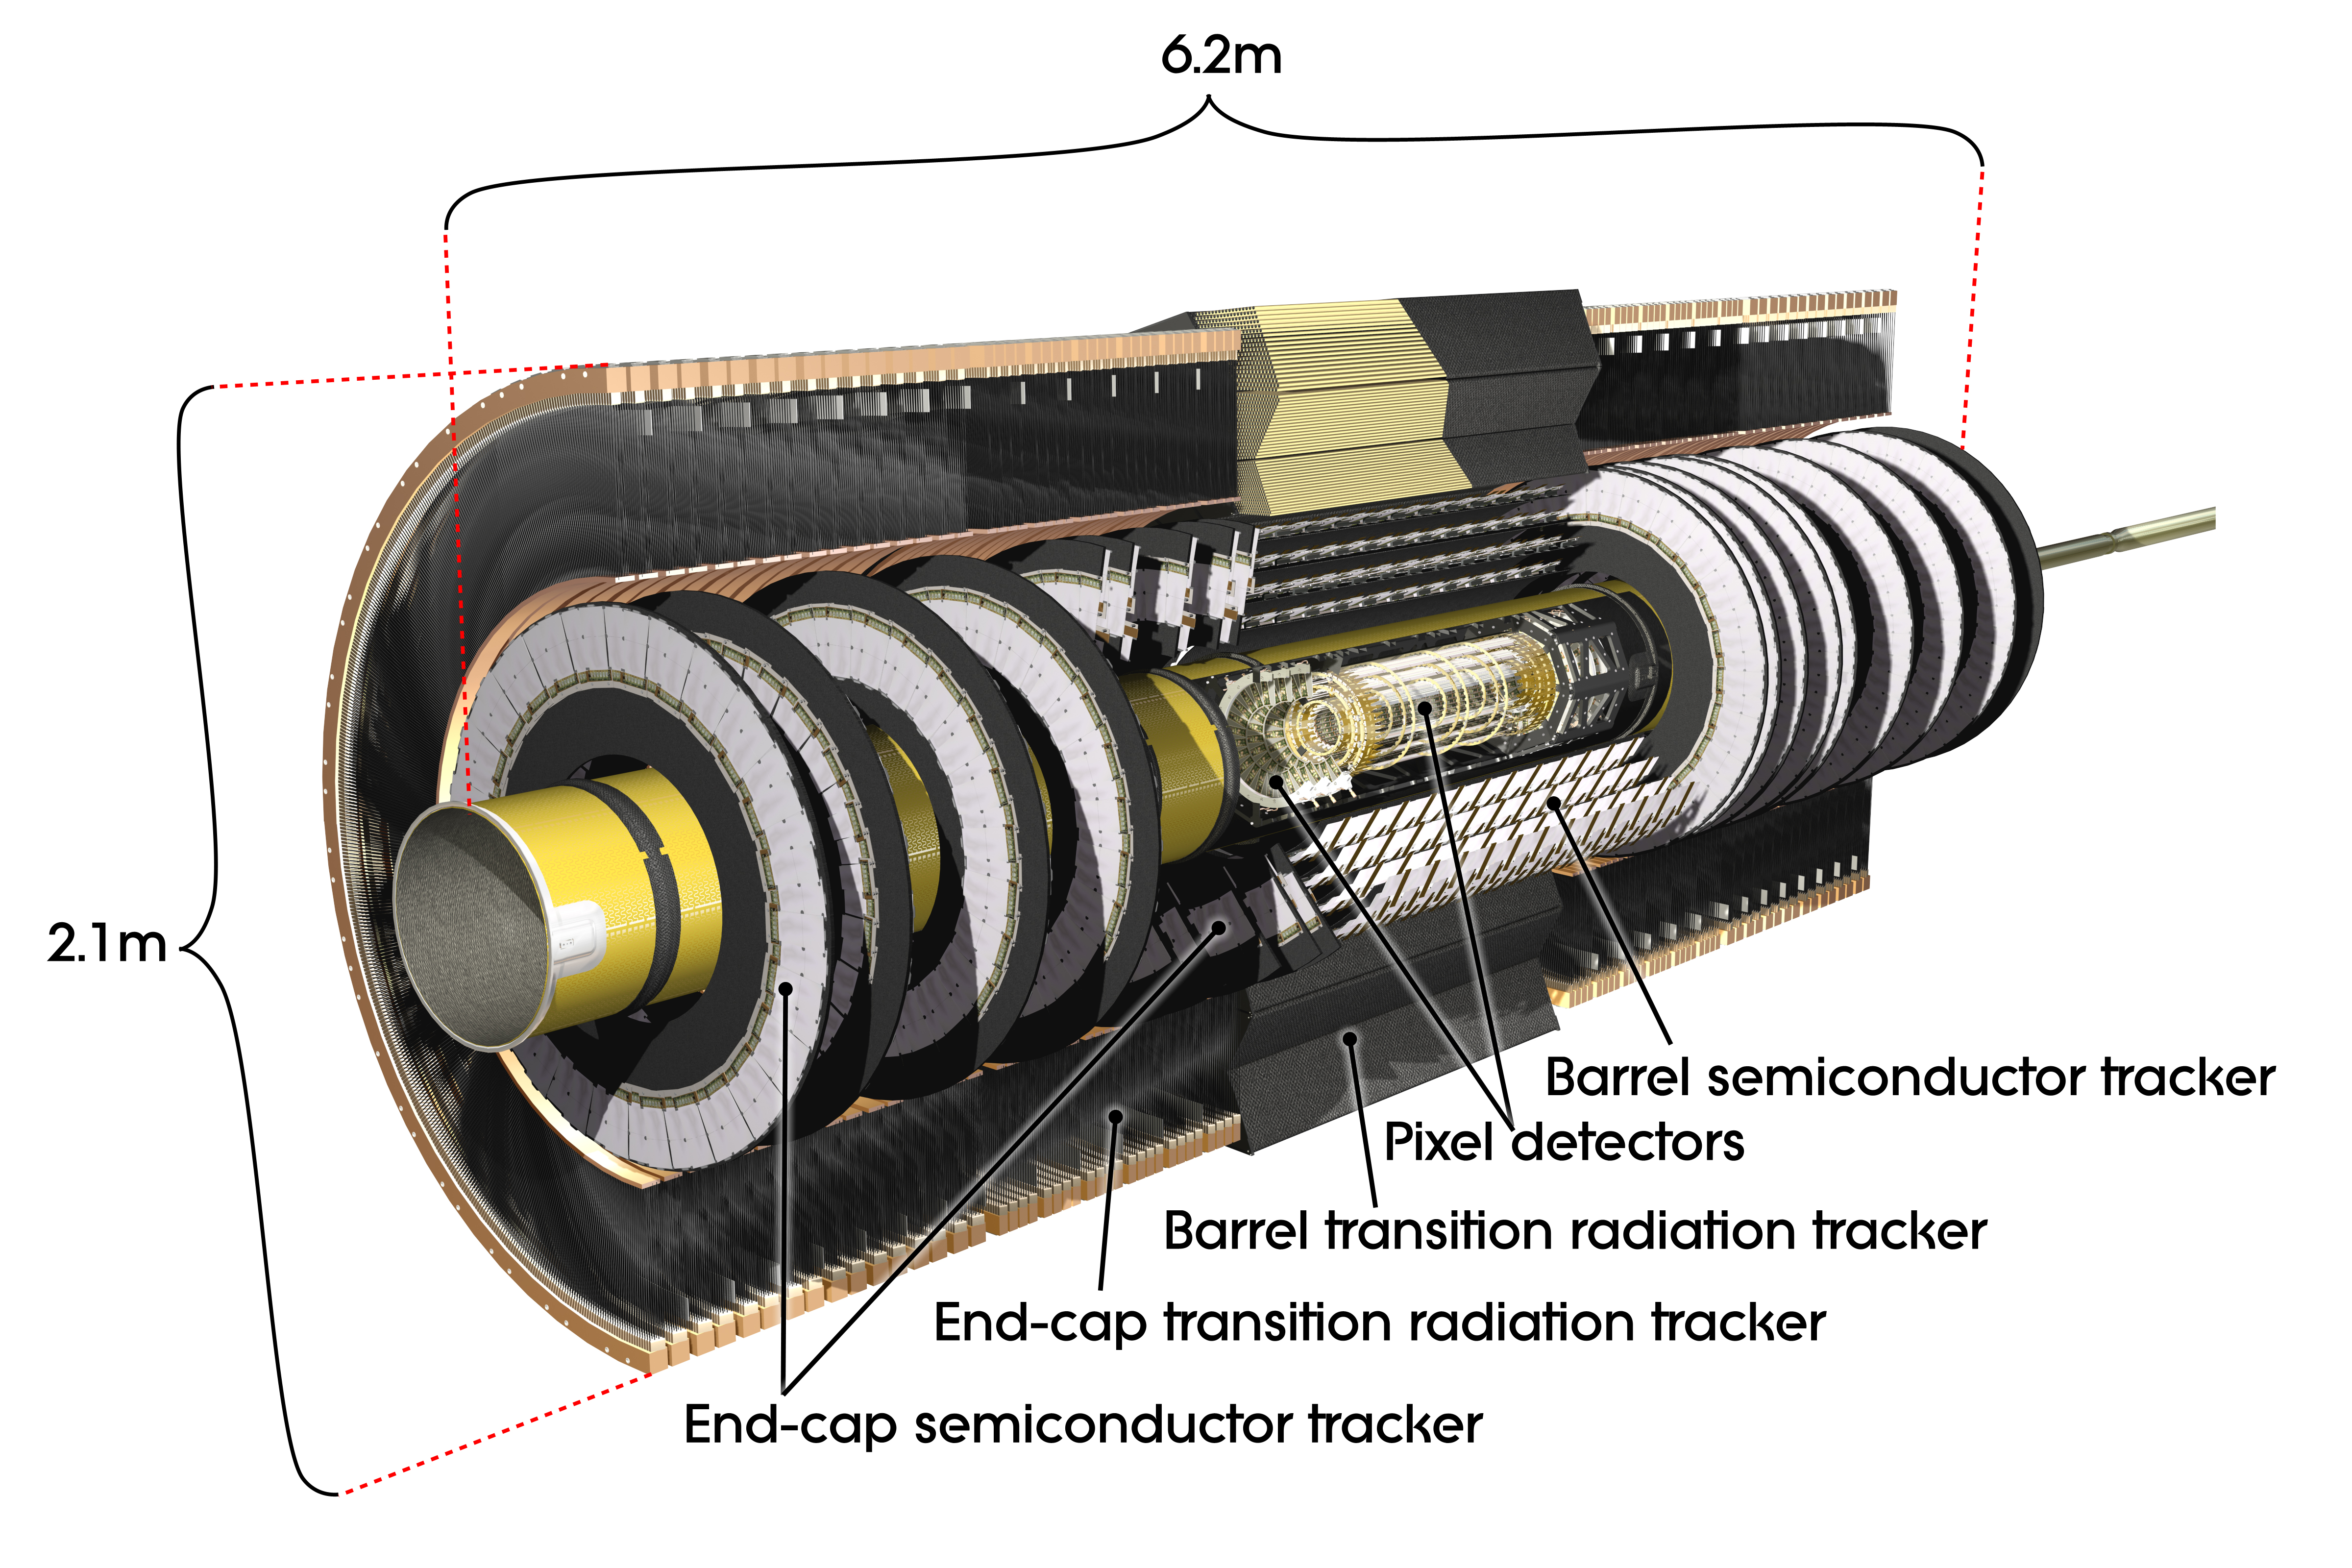
\includegraphics[width=.7\textwidth]{Inner-detector}
  \caption[ATLAS inner detector]{Computer generated image of the ATLAS inner
detector~\cite{ATLAS-inner-det}.}%
  \label{fig:ATLAS-inner-det}
\end{figure}

With the exception of the TRT the tracking sub-systems are silicon based
detectors. The silicon detection medium acts as a reverse bias diode. Charged
particles incident on the silicon cause ionisation in the depletion layer. The
products of this ionisation are electons and holes (excess pockets of positive
charge in the silicon) which produce a signal that must be handled by a
read-out system. The signal is referred to as the collected charge.
Application-specific integrated circuits (ASICs) are used to readout the signal
performing the analogue to digital conversion. The combination of the detection
medium, readout system and the printed circuit board (PCB) on which they are
joined is referred to as a module.

\subsubsection{Pixel Detectors}

There are four layers of pixel detectors that are the closest components of the
ID to the beam-pipe. Pixel detectors are silicon detectors where the diodes are
rectangular in shape, giving the benefit of being able to resolve hits
in two directions. The design originally had three layers, each 250~$\mu$m
thick with 50~$\mu$m by 250~$\mu$m pixels, of oxygen doped n-type silicon
crystals. During LS1 a fourth layer, closest to the beam-pipe (which was also
replaced for a smaller radius version) was added. This layer is known as the
insertable B-layer (IBL)~\cite{IBL-TDR}, the motivation for its addition was to
counteract degradation of original performance of the ID due to irreversible
damage by radiation. As well as the inclusion of the IBL, performance degradation
is mitigated by increasing the bias voltage across the pixels from 100~V (their
starting voltage) to up to 600~V. Additionally the IBL being closer to the
beam-pipe allows for interaction vertices to be measured more precisely. The
need for better reconstruction of vertices is motivated by their role in the
performance of algorithms that classify jets of activity in the detector that
are initiated by B-hadrons. This is where the IBL gets its name. There are no
pixel detectors in the end-caps. Each pixel is small in size which means many
can fit on one module, all requiring their own conductor for readout. The
solution to this challenge is to use a complex process known as bump bonding,
which is both expensive and time consuming.

\subsubsection{Semiconductor Tracker}

Next closest to the beam-pipe is the SCT whose modules have long thin strip
shaped diodes. The strips provide high resolution in only a single direction. In
contrast to the n-type silicon of the pixels, the strips are made from p-in-n
type silicon. Each SCT module is comprised of two back to back silicon
rectangles such that the orientation of the strips are offset by a small angle
in order to improve coverage. Each strip is covered with metalisation on top.
The strips are separated by a distance of 80~$\mu$m. A rather old and dirty SCT
module left over from the quality control testing stage of production that took
place at Queen Mary University of London can be seen in
figure~\ref{fig:strip-module}. As can be seen in the figure the SCT modules are
wire bonded to their ASICs which is cheaper than the bump bonding used on the
pixel modules.
\begin{figure}[ht]
  \centering
  \includegraphics[width=.7\textwidth]{sct-module}
  \caption[ATLAS long strip module]{An image of an SCT long strip module
    mounted in a rig for testing at Queen Mary Univesity of London.}
  \label{fig:strip-module}
\end{figure}
In order to calibrate the response of the strips a 100~M$\Omega$ poly-silicon
resistor is located at the end of each strip. Figure~\ref{fig:sct-close} shows an
image of the snake-like structure of a poly-silicon resistor from the end of an
SCT module.
\begin{figure}[ht]
  \centering
  \includegraphics[width=.7\textwidth]{sct-close}
  \caption[ATLAS strip close-up]{A close up image of the end of an SCT sensor in
    which the snake-like poly-silicon resistors are visible as a yellowish
    coloured structure at the end of each strip. This image was taken with a
    high resolution automatic area scanner commissioned by the
    author~\cite{itk-scanner} in order to take full scans of strip sensors
    during the production of the ATLAS Inner Detector upgrade known as the Inner
    Tracker (ITk)~\cite{itk-tdr, itk-strips-tdr}.}
  \label{fig:sct-close}
\end{figure}
The modules come in two different designs, short strips and long
strips with the short strips forming the layer closest to the pixel detectors
and the long strips on the outside. The original operating bias voltage was
150~V but again due to radiation exposure this will raise to up to 350~V over
time as necessary. There are four layers of semiconductor trackers in the barrel
arranged so that sensors have a tilt with respect to a perfect coaxial cylinders
of approximately 11$\degree$. This tilt increases the amount of material that
particles will travel through and is optimized to the geometry of the detector.
Similarly the end-cap modules are arranged in petal like structures, with a
number of different geometric designed based on the position within the end-cap.

\subsubsection{Transition Radiation Tracker}

The last part of the ID is the TRT. The primary role of the TRT is to aid
electron identification by measurement of transition radiation. This is useful
in distinguishing between electrons and charged hadrons which can leave similar
signatures in the calorimeters and whose tracks are otherwise hard to
distinguish. The TRT is mostly made up of polyimide drift tubes with a diameter
of 4~mm. The drift tubes are filled with a gas mixture whose majority
constituent is xenon. These tubes operate with a voltage of -1530~V and are
contained within a carbon fibre support structure. Scintillating fibres and
foils lie between the drift tubes which create the transition radiation.  The
geometric layout of the tubes is optimised individually for the barrel and
end-caps.

\subsubsection{Tracker Performance}
The resolution with which track impact parameters can be determined gives a good
picture of the tracker performance. A comparison of the impact parameter
resolution between 2012 and 2015 is shown in figure~\ref{fig:impact-param-reso}
which shows significant improvement in the resolution in that time period.
\begin{figure}[ht]
  \centering
  \includegraphics[width=.8\textwidth]{impact-param-performance}
  \caption[ATLAS impact parameter resolution (2012 v.s. 2015).]{The resolution
    of the impact parameters $d_0$ and $z_0$ plotted as a function of
    $p_T$~\cite{ATLAS_RUN_2_PERF}. The black circles are data from Run-1 and the
    red filled circles are from one year of Run-2, 2015.}
  \label{fig:impact-param-reso}
\end{figure}

Figure~\ref{fig:track-eff} shows the tracking efficiency in 2015, more detail on
the track reconstruction performance of the inner detector can be found
in~\cite{ATL-PHYS-PUB-2015-018}.
\begin{figure}[ht]
  \centering
  \includegraphics[width=.8\textwidth]{track-recon-eff}
  \caption[ATLAS track reconstruction efficiency.]{The ATLAS tracker
    reconstruction efficiency in 2015. Where the efficiency is the number of
    reconstructed tracks over the number of generated particles in the simulated
    event~\cite{ATL-PHYS-PUB-2015-018}.
  }
  \label{fig:track-eff}
\end{figure}


\clearpage
\newpage

\subsection{Calorimeters}%
\label{sec:calo}

The purpose of the calorimeters is to measure the total energy of particles that
pass through their volume. This is achievable only if the calorimeter stops the
particle completely. A desirable side effect is that they also act as a barrier
to stop particles passing through to the muon spectrometers.Of course this
means necessarily that muons pass through the calorimeters. There are two
calorimeter systems in ATLAS, the electromagnetic calorimeter (ECAL) and the
hadronic calorimeter (HCAL). The calorimeters are not immersed in a significant
magnetic field compared to the rest of ATLAS as seen in the heat map of
figure~\ref{fig:ATLAS-magnets}. The geometric layout of the calorimeter systems,
as well as the location of specific components can be seen in
figure~\ref{fig:ATLAS-calo}, in which the ID can also be seen (greyed out).
Information from the two calorimeters is used in conjunction for any particles
whose decay products propagate through both volumes. Both calorimeters are split
up into cells of material that are used to determine the position of decay
products in the detector.
\begin{figure}[ht] \centering 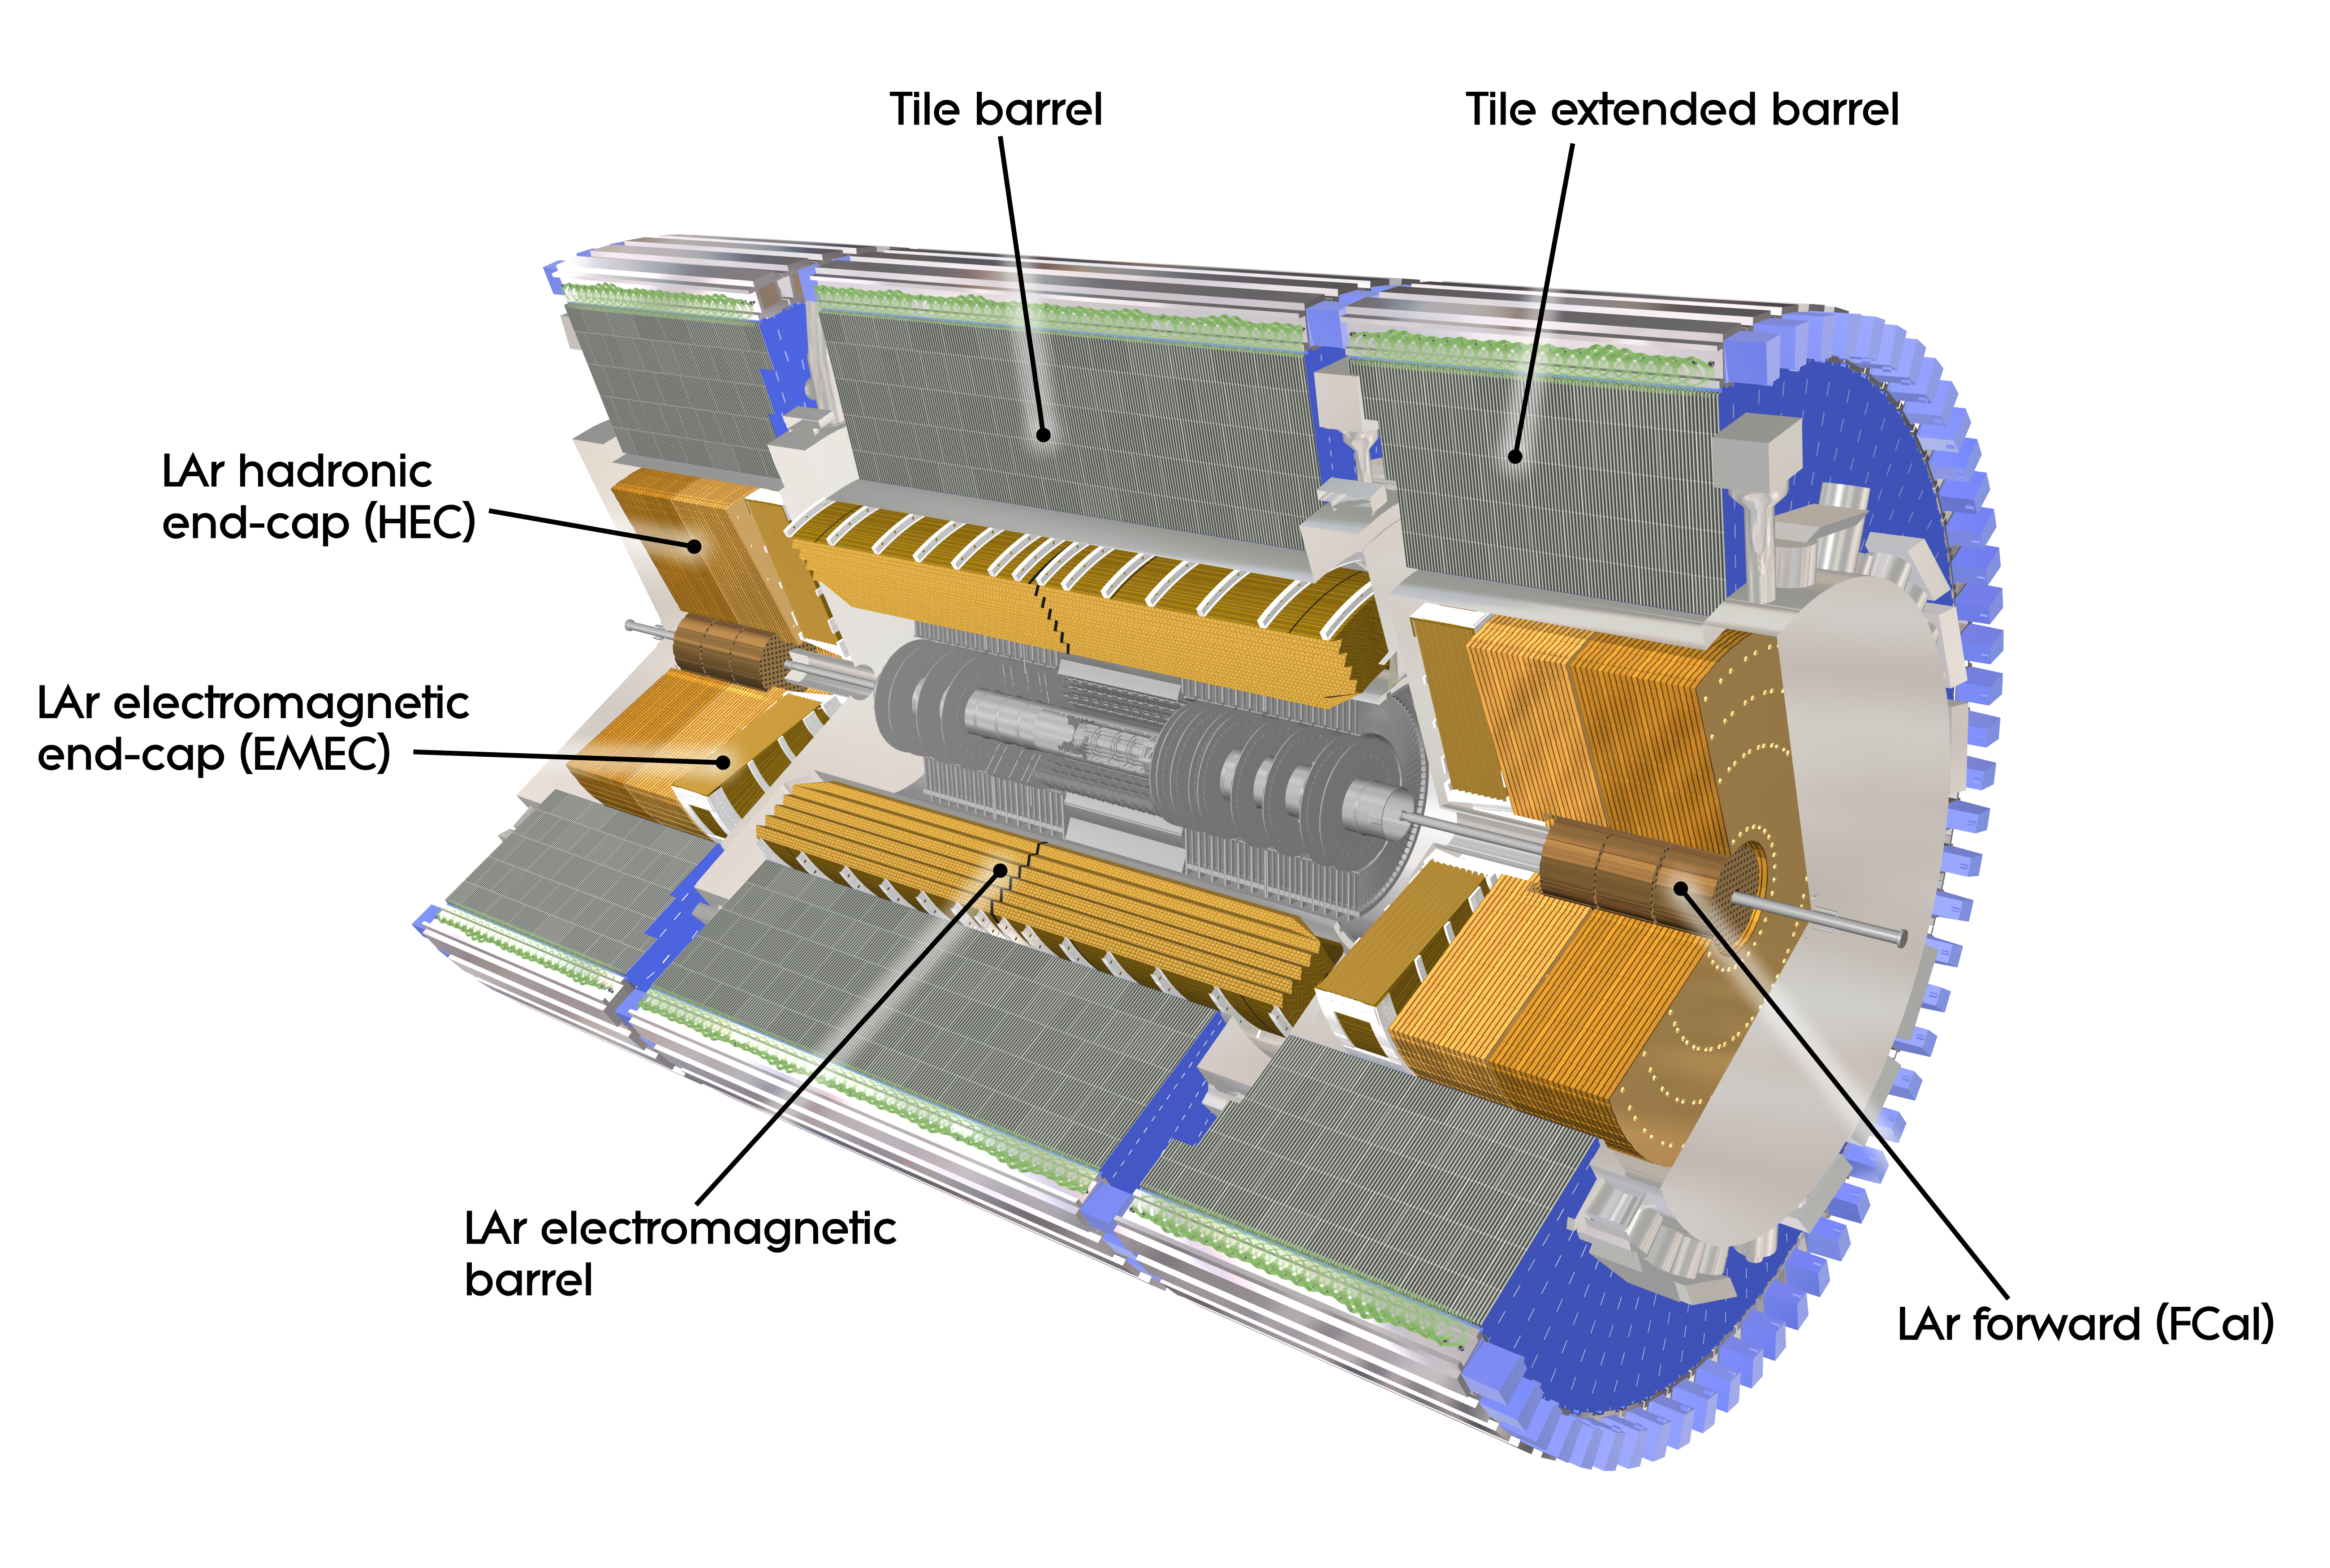
\includegraphics[width=.7\textwidth]{ATLAS-calo}
  \caption[ATLAS Calorimeter]{Computer Generated image of the ATLAS
calorimeter~\cite{ATLAS-calo-fig}.}%
  \label{fig:ATLAS-calo}
\end{figure}

High energy physics calorimeters function by measuring the shower
of particles that are produced as a result of the incident particle losing its
energy. Both calorimeters in ATLAS are sampling calorimeters, meaning that they
are comprised of alternating layers of absorber and detection medium. The purpose
of the absorber medium is to provide a material in which particle showers evolve
rapidly over a short distance, though they are in general not sensitive to
measuring those showers. The detection medium or active material is used to then
measure those showers.

In general a good calorimeter will have the following properties: it should be
hermetic, meaning that there are no gaps for particles to escape through without
being measured. It should have a fast response time, to keep up with the rate of
collisions (actually the rate of the trigger see the following section). It
should be radiation tolerant in order to perform over a long period of time. It
should be able to measure energy to a high resolution in order to resolve
resonances over backgrounds and have a high granularity of cells in order to
accurately determine the position of energy deposits (and aid particle
identification). High energy resolution is greatly aided by not having anything
in front of the calorimeter which may change an incident particle's energy
before it strikes the calorimeter itself. This requirement is therefore somewhat
at odds with having a detector that has good $p_{\mathrm{T}}$ resolution for
electrons, positrons and photons (muons go all the the way through the
calorimeter anyway) due to the process by which $p_{\mathrm{T}}$ is measured
becoming more precise with a longer ``lever-arm'' distance $L$ as seen in
figure~\ref{fig:sagitta} and equation~\ref{eq:sagitta}. A large tracker makes
the calorimeter much more expensive in a barrel shaped detector as the amount of
material required increases with the square of the radius of the tracker.

\subsubsection{Electromagnetic Calorimeter}
The ECAL is primarily concerned with measuring the energy of electrons,
positrons and photons. Theses particles primarily interact with the
electromagnetic force and so produce electromagnetic showers when they lose
their energy. The ECAL resides closer to the interaction point than the HCAL and
has liquid argon (LAr) as its active material. LAr is a good choice for the
calorimeter which is closer to the interaction point as it is naturally
resistant to damage by radiation. The absorber of the ECAL is lead, which is
suitable as it has a high number of nucleons ($Z$) and the radiation
length\footnote{The radiation length $X_{0}$ is the thickness of material that
reduces the energy of an electron by a factor of $e$ the natural number, but is
also used for other particles.} of a given shower is inversely proportional to
$Z^2$. An applied electric field causes ions produced in the EM shower to drift
in such a way that the signal induced is proportional to the energy deposited by
the incident particle.

\subsubsection{Hadronic Calorimeter} The HCAL end-caps use a LAr active material
like the ECAL. The absorber is copper instead of lead and the dimensions are
more suited to hadronic particle showers as opposed to electromagnetic. As noted
before, LAr is naturally radiation hard which is why it is used in the end-caps
which see more radiation than the barrel regions due to almost all of the
momentum of the colliding bunches of particles being in the axis of the
beam-pipe. The barrel section of the hadronic calorimeter is made from
scintillating tiles of active material interspersed with steel as an absorber.
Scintillation is the process by which a scintilation medium produces light when
particles travel through it. The amount of light produced is proportional to the
energy of the incident particle that initiated the shower. In order to convert
the light into a digital electrical signal photo-multiplier tubes (PMTs) are
used. PMTs are able to measure very small amounts of light, even the incidence
of a single photon. This is achieved by initially exploiting the photo-electric
effect whereby the incident photon knocks an electron from a metallic part of
the PMT. The current produced by this electron is then multiplied by a very
large factor (up to $10^8$ for some PMTs) by a series of dynodes (electrodes in
vacuum that produce secondary emission).

\subsubsection{Calorimeter Performance}
Put calorimeter performance here: LAr performance, 

\subsection{Muon Spectrometers}%
\label{sec:muon}

Surrounding the calorimeters are the muon spectrometers, which form the
outermost layer of the detector. Though muons are charged leptons just like
electrons, their specific properties mean that dedicated muon spectrometers are
required to detect them. Muons deposit far less energy per distance traveled
than other particles meaning that they punch through most materials with ease.
As can be seen in figure~\ref{fig:ATLAS-muon} the components of the muon
spectrometers are the thin-gap chambers, cathode strip chambers, resistive plate
chambers and monitor drift tubes. The barrel and end-cap toroid magnets immerse
the muon spectrometers in a magnetic field which at its peak (visible in
figure~\ref{fig:ATLAS-magnets}) has a strength of 4~T. Despite a stronger
peaking magnetic field than in the solenoid, observed muon tracks are often far
less curved than that of their lighter cousins, the electrons. Muons do leave
tracks in the ID and also deposit small amounts of energy in the calorimeters.
Tracks in the muon spectrometers are matched up to tracks in the ID with the aid
of the location of energy deposits in the calorimeters if possible. Tracking
information for muons is used in algorithms such as overlap removal, which
removes muons from jets that they have been erroneously associated with by
matching the muon with its ID track.
\begin{figure}[ht]
  \centering
  \includegraphics[width=.7\textwidth]{ATLAS-muon-spec}
  \caption[ATLAS muon subsystem]{Computer generated image of the ATLAS Muons
    subsystem~\cite{ATLAS-muon-fig}.}%
  \label{fig:ATLAS-muon}
\end{figure}

\subsection{Missing Transverse Energy Resolution}
Plot of MET resolution callback to part where we say MET depends on all bits of the detector.

\subsection{Trigger Systems}%
\label{sec:trigger}

The trigger systems in ATLAS allows data to be recorded only when an event meets
certain criteria. It would be impossible to read out every interaction that
occurs in the detector. The reason for this is that the geometric constraints of
the detector mean that there is only a small space available for readout wires,
as detection medium needs to be prioritized for sensitivity and technology
limits the data rate that one can achieve through a cable of fixed area. The
trigger system comes in two parts, a hardware component referred to as level one
(L1) and software component referred to as the high level trigger (HLT). The L1
system is comprised of the L1 calorimeter (L1Calo) trigger which operates by
searching for clusters of energy in the calorimeters and the L1 muon (L1Muon)
system which coincidences in the muon systems. A third system L1 topological
(L1Topo) uses regions of interest built from the L1Calo and L1Muon data which
are passed to central trigger processors for selection. The various limitations
of the hardware mean that these selections must be passed up to the next level
of triggering, the HLT in a time window of 2.5~$\mu$s. The HLT takes information
from the L1 systems and uses faster versions of an offline style analysis in
order to select or reject events for readout. The rate of the HLT was about 1.2
kHz on average over the period of data taking relevant to this measurement. In
order for a trigger to fire an event must pass fully all of the requirements of
one of the algorithms defined by an extensive trigger menu. More information
about the triggers used in the \VHbb\ analysis will be given in a later chapter.
